\section{Point-Mass Guidance Prototype}

The second stage used the MANSUP point-mass model to test two horizontal engagement geometries. At this level, the model is mainly useful for guidance logic: pre-programmed flight, seeker limits and the switch to terminal homing.

\subsection{Base Model and Changes}

The course Simulink model remained as the base, with edits concentrated in the control subsystem:

\begin{itemize}
    \item the \(X\)-\(Z\) plane was interpreted as the horizontal plane;
    \item \(Z\) was treated as horizontal lateral displacement;
    \item altitude \(10~\text{m}\) was used only for atmosphere calculation;
    \item a pre-programmed turn law was added for off-boresight launch;
    \item terminal guidance was allowed only when the target was within the required distance and seeker cone.
\end{itemize}

The pre-programmed command was based on the angular error between the missile heading and the line of sight:

\[
    G_{pre}=K_{pre}\left[\operatorname{atan2}(\Delta z,\Delta x)-\gamma\right].
\]

\begin{figure}[H]
\centering
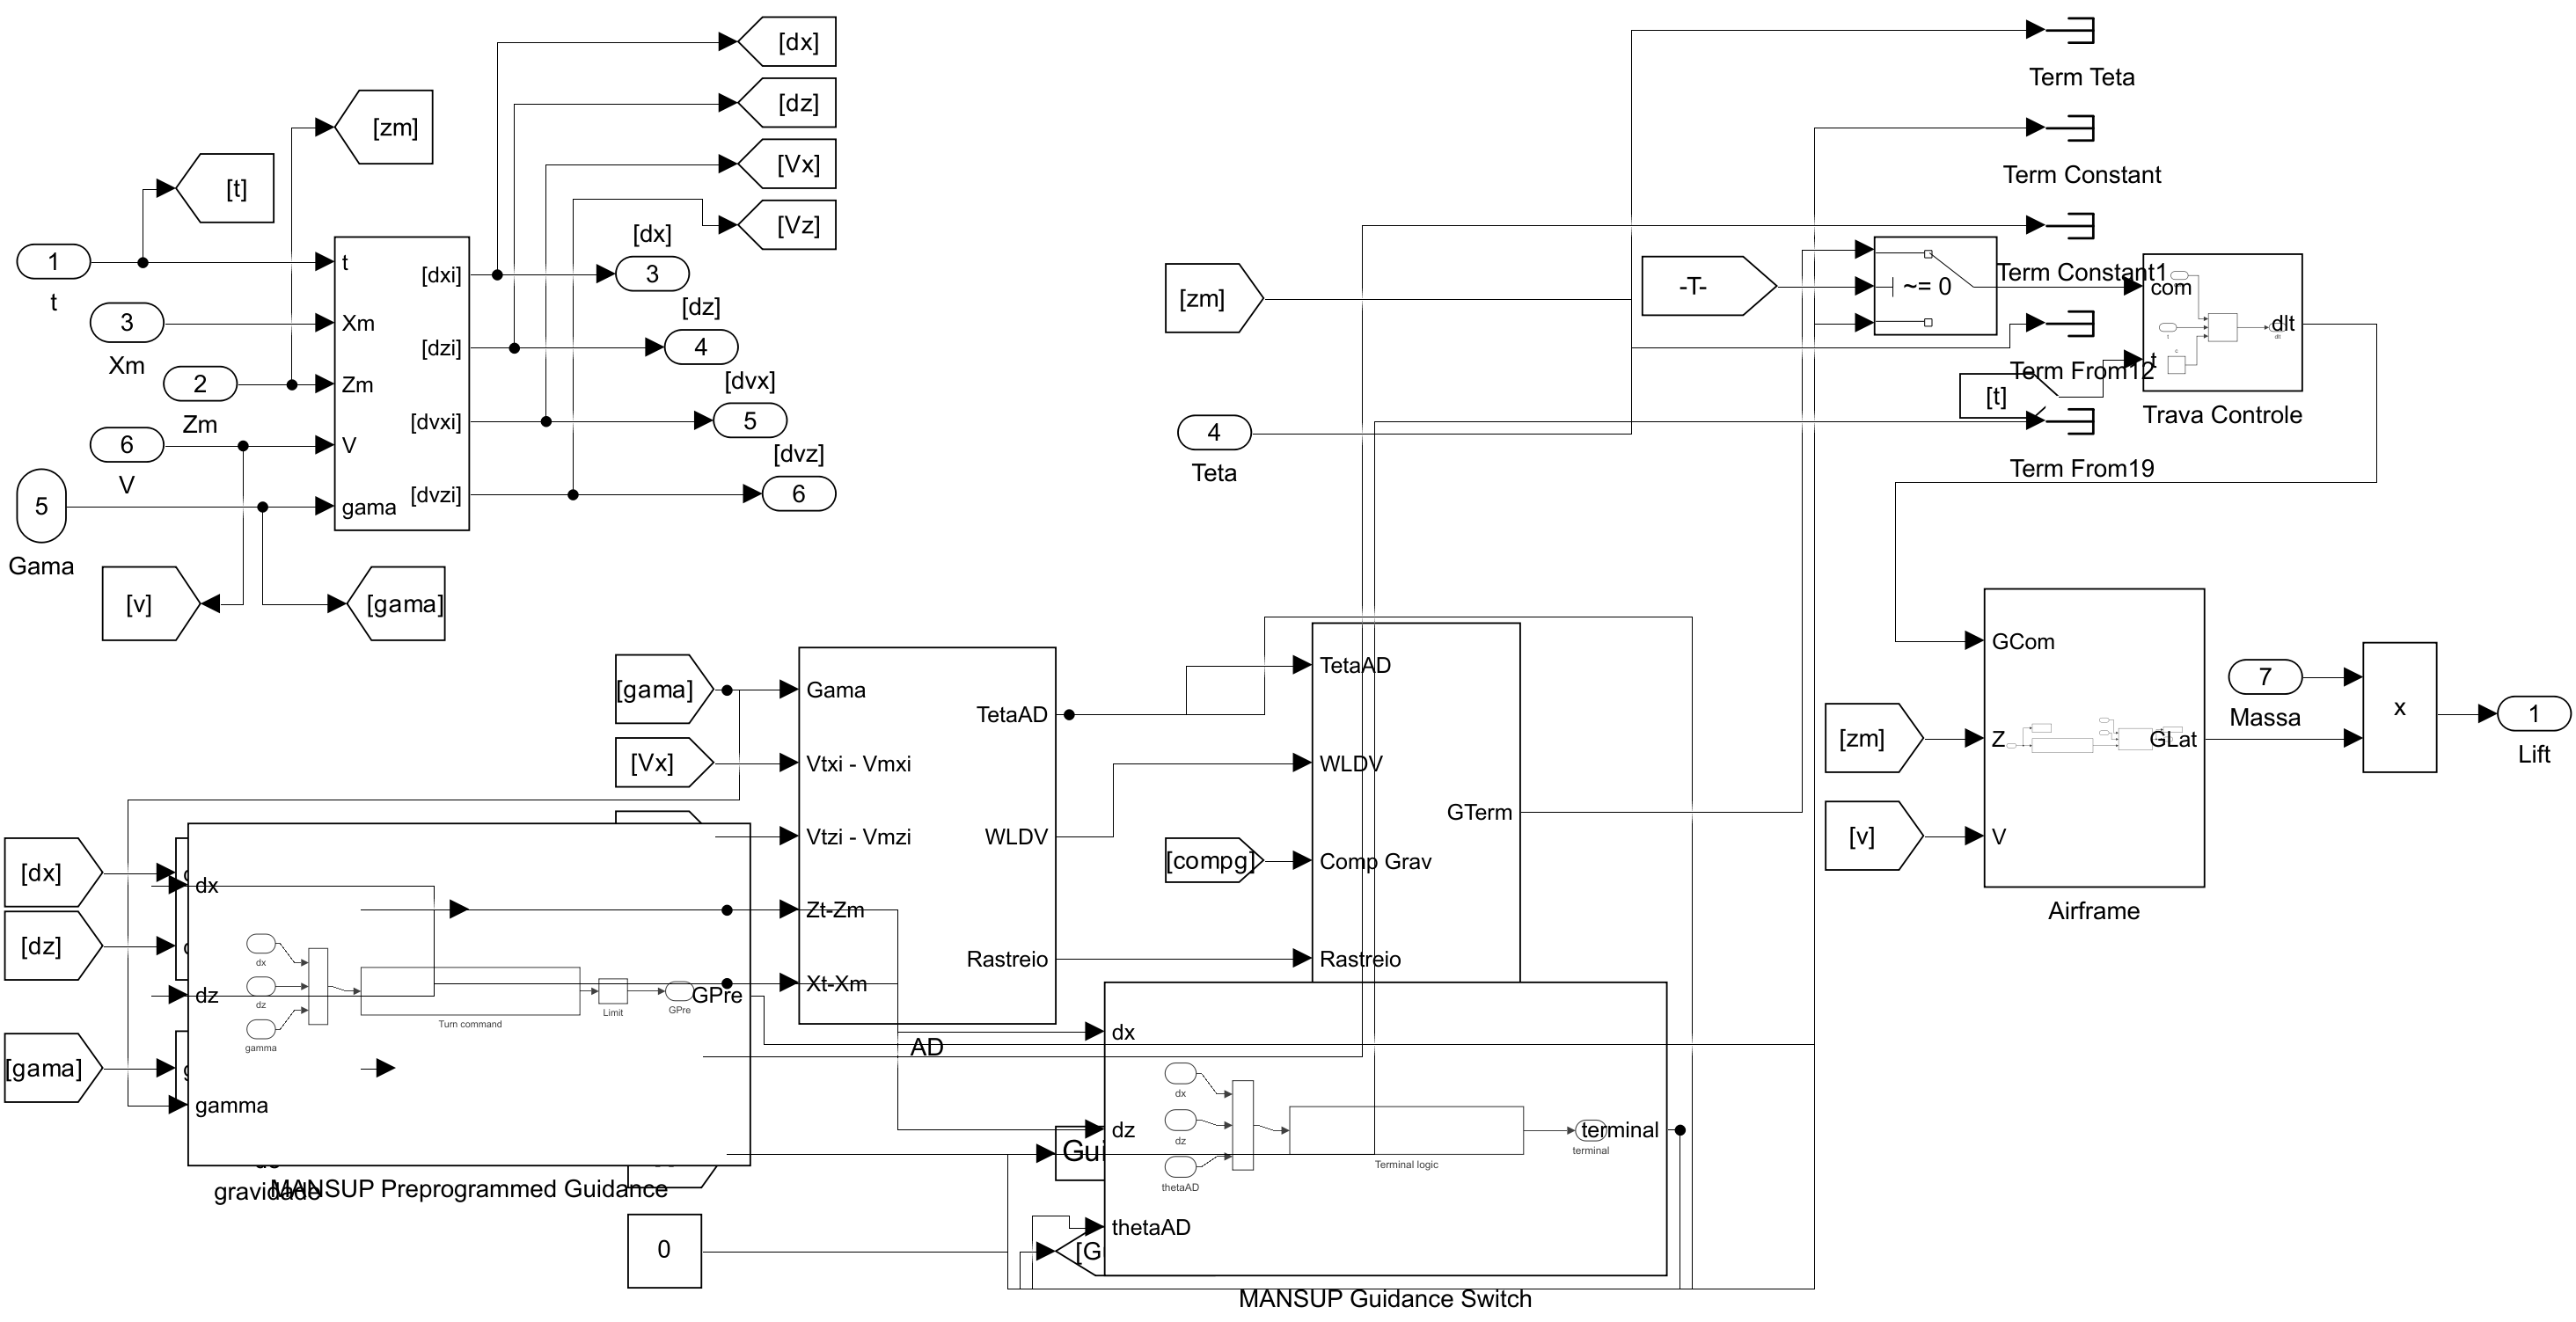
\includegraphics[width=0.92\textwidth]{figures/model_control.png}
\caption{Modified control subsystem in the point-mass Simulink model.}
\end{figure}

\begin{figure}[H]
\centering
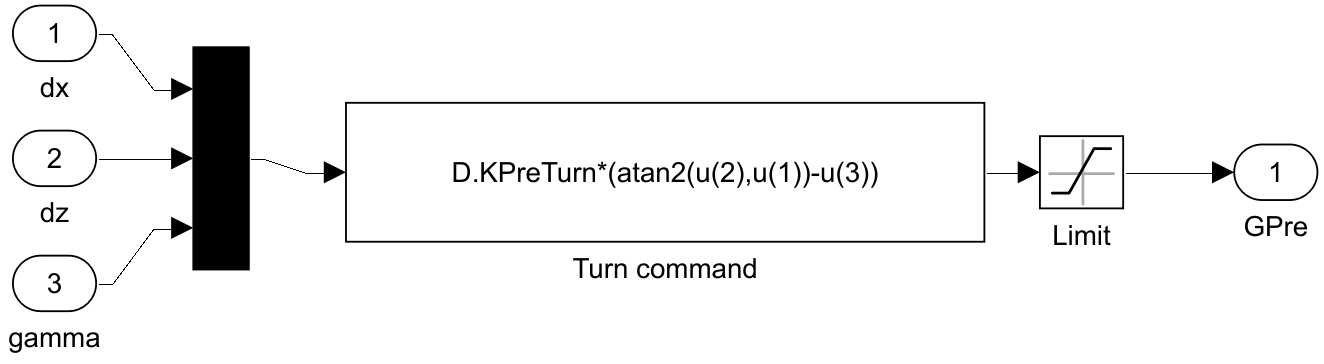
\includegraphics[width=0.75\textwidth]{figures/model_preprogrammed.png}
\caption{Pre-programmed guidance block used to generate the horizontal turn command.}
\end{figure}

\subsection{Guidance Cases}

\begin{table}[H]
\centering
\caption{Point-mass simulation cases.}
\begin{tabular}{p{0.18\textwidth}p{0.34\textwidth}p{0.38\textwidth}}
\toprule
Case & Initial condition & Terminal logic \\
\midrule
1 & Target at \(65~\text{km}\), launch bearing \(0^\circ\) & Terminal guidance starts at \(20~\text{km}\) from the target. \\
2 & Target at \(15~\text{km}\), launch bearing \(90^\circ\) & Seeker is on from launch, but terminal mode waits until target enters the \(40^\circ\) cone. \\
\bottomrule
\end{tabular}
\end{table}

\begin{table}[H]
\centering
\caption{Point-mass simulation results.}
\begin{tabular}{lcc}
\toprule
Result & Case 1 & Case 2 \\
\midrule
Terminal guidance start & \(146.35~\text{s}\) & \(13.95~\text{s}\) \\
Range at terminal start & \(19.997~\text{km}\) & \(12.680~\text{km}\) \\
Flight time & \(214.90~\text{s}\) & \(58.95~\text{s}\) \\
Final range & \(500.0~\text{m}\) & \(549.0~\text{m}\) \\
Final speed & \(284.4~\text{m/s}\) & \(305.0~\text{m/s}\) \\
\bottomrule
\end{tabular}
\end{table}

\begin{figure}[H]
\centering
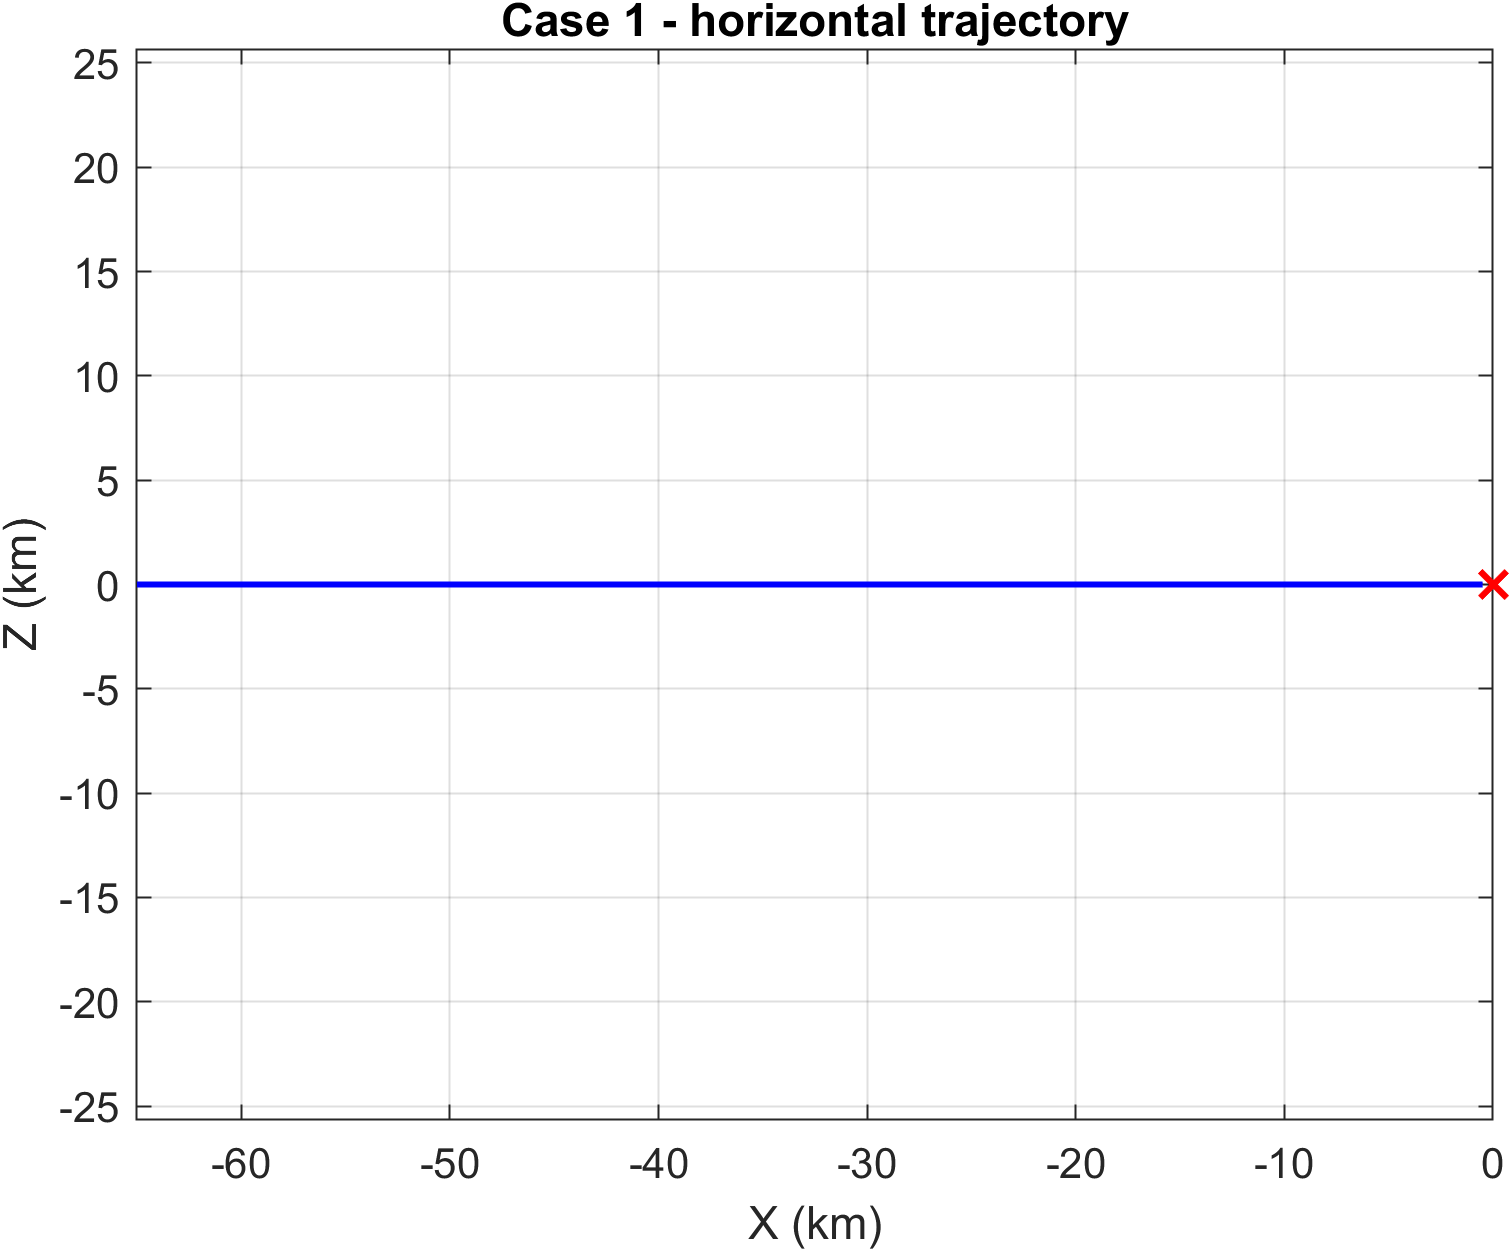
\includegraphics[width=0.82\textwidth]{figures/case1_trajectory.png}
\caption{Case 1 horizontal trajectory.}
\end{figure}

\begin{figure}[H]
\centering
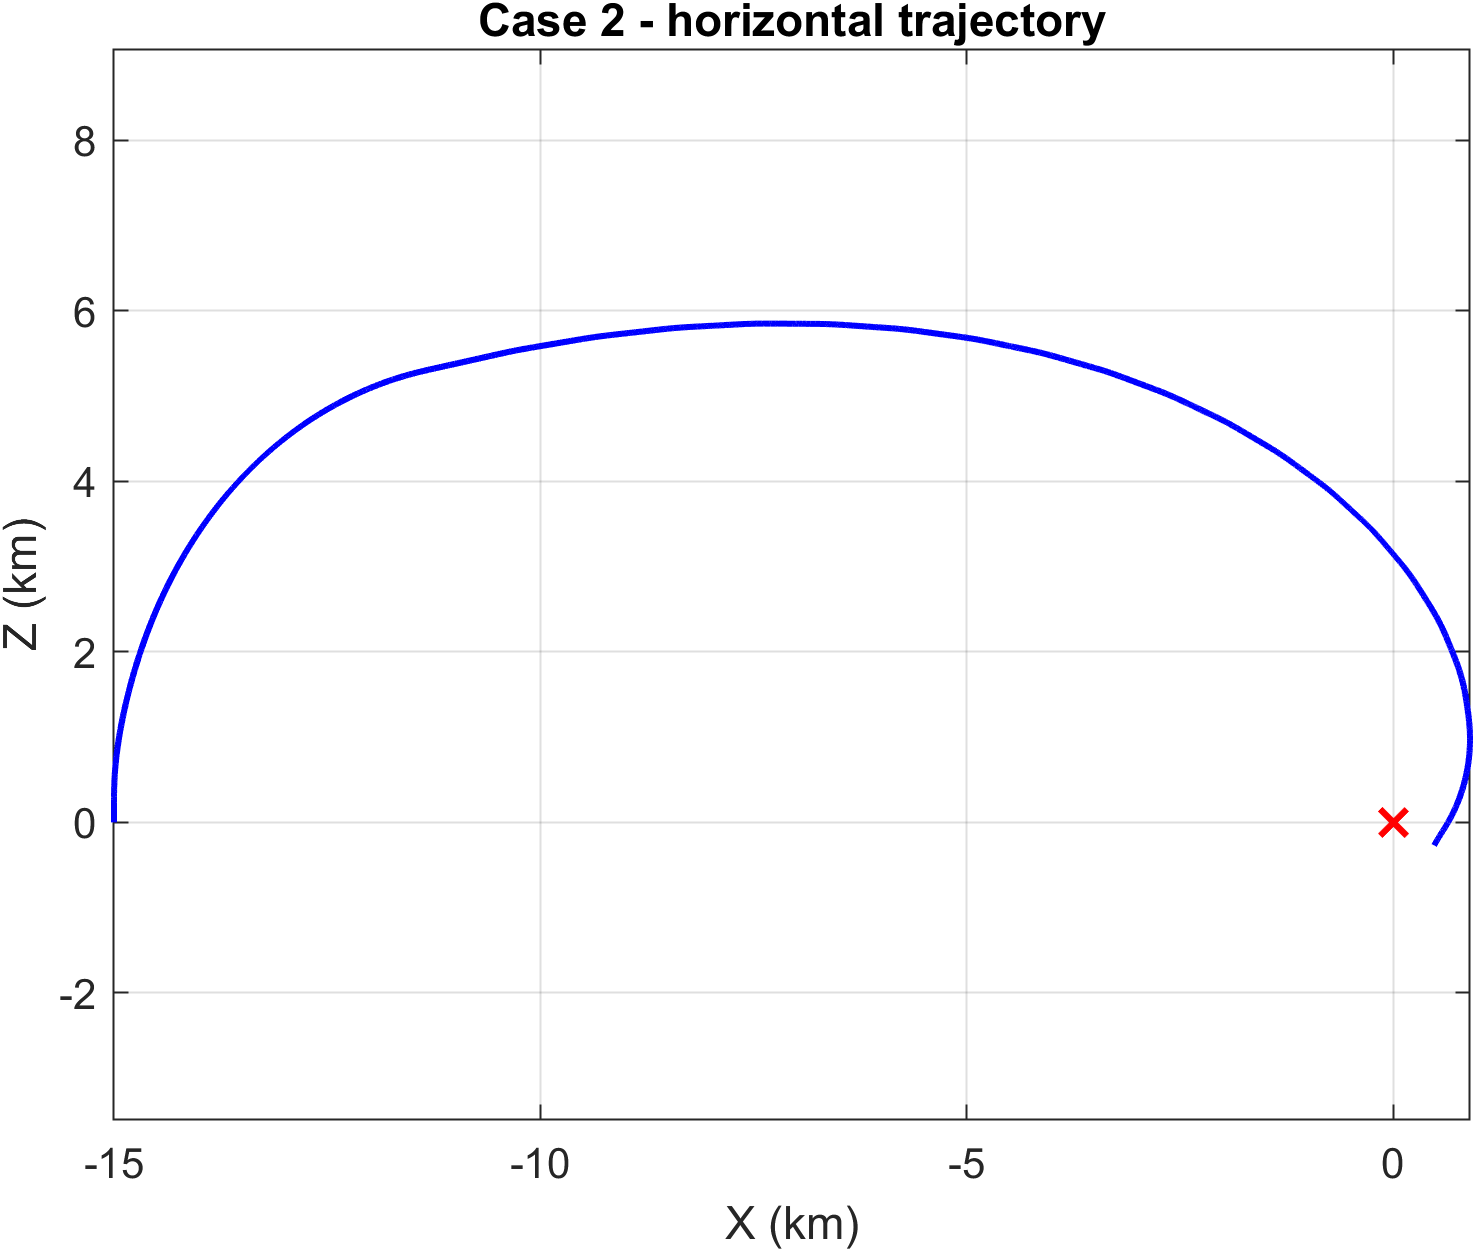
\includegraphics[width=0.82\textwidth]{figures/case2_trajectory.png}
\caption{Case 2 horizontal trajectory with pre-programmed turn before terminal guidance.}
\end{figure}

The switching logic uses two conditions: the seeker must be active and the target must be inside the allowed field of view. This is the important point in Case 2, because the seeker starts active while the target is still outside the \(40^\circ\) cone.
